\section{Bindings}
\label{sec:Bindings}

In addition to Java, COMPSs supports the execution of applications written in other languages by 
means of bindings. A binding manages the interaction of the not-Java application with the COMPSs 
Java runtime, providing the necessary language translation.

The next subsections describe the language bindings provided by COMPSs.

\subsection{C/C++}

COMPSs provides a binding for C and C++ applications. The new C++ version in the current release 
comes with support for objects as task parameters and the use of class methods as tasks.

\subsubsection{Programming Model}

\paragraph{Task Selection}
As in Java language the user must write the task selection like an ``interface''. In this case 
the interface file has the same name as the main application file plus the suffix ``idl'', 
i.e. Matmul.idl, where the main file is called Matmul.cc.

\begin{lstlisting}[language=C++]
interface Matmul
{
      // C functions
      void initMatrix(inout Matrix matrix,
                      in int mSize,
                      in int nSize,
                      in double val);
                      
      void multiplyBlocks(inout Block block1,
                          inout Block block2,
                          inout Block block3);
                          
      // C++ class methods
      void Block::multiply(in Block block1,
                           in Block block2);
                           
      static Matrix Matrix::init(in int mSize,
                                 in int bSize,
                                 in double val);
};
\end{lstlisting}

The syntax of the interface file is shown in the previous code. Tasks can be declared as classic 
C function prototypes, this allow to keep the compatibility with standard C applications. 
In the example, initMatrix and multiplyBlocks are functions declared using its prototype, 
like in a C header file, but this code is C++ as they have objects as parameters (objects of 
type Matrix, or Block).

A class method can be also a task, and it is declared using its signature. In the example, 
Block::multiply and Matrix::init are class methods. In this example, C functions encapsulates 
object method calls, as we will see later.

The grammar for the interface file is as follows:

\begin{lstlisting}[language=bash]
["static"] return-type task-name ( parameter {, parameter }* );

return-type = "void" | type

ask-name = <qualified name of the function or method>

parameter = direction type parameter-name

direction = "in" | "out" | "inout"

type = "char" | "string" | "int" | "short" | "long"
    | "float" | "double" | "boolean" | "File" | class-name

class-name = <qualified name of the class>
\end{lstlisting}

       
\paragraph{Value and Object return}
Notice that returning a value or an object is now supported, this means a ``void'' value, a value 
of a primitive type (an int, long, float, etc.), or an object of a class, can be returned from a 
function or method.

{\bf IMPORTANT:}

In C/C++ the default policy is to make a copy of the value or object when it is returned [A = foo();], 
and this copy (A) is a new position in memory whom reference or address is not possible to know before 
the return statement.

As the binding can’t know such reference before leaving the task execution (foo) it must do a 
synchronization before the return statement for the correct value to be copied when returning. 
This is called an explicit synchronization.

Alternatively, the return of a value or an object can be done also by mean of an out or inout parameter, 
and no explicit synchronization is needed because the reference is passed to the binding in this case 
using de \& operator [foo(\&A);].

\paragraph{Main Program}
The main program is a sequential code written in C++ that launches tasks to be executed in parallel 
and may have several data-synchronization points or none.

\begin{lstlisting}[language=C++]
#define %*{\bf DEBUG\_BINDING }*)
#include %*{\bf "Matmul.h" }*)
#include "Matrix.h"
#include ""Block.h"
int N; //MSIZE
int M; //BSIZE
double val;
int main(int argc, char **argv)
{
      Matrix A;
      Matrix B;
      Matrix C;

       N = atoi(argv[1]);
       M = atoi(argv[2]);
      val = atof(argv[3]);

      %*{\bf compss\_on(); }*)

      A = Matrix::init(N,M,val);

      initMatrix(&B,N,M,val);
      initMatrix(&C,N,M,0.0);

      cout << "Waiting for initialization...\n";

      %*{\bf compss\_wait\_on(B); }*)
      %*{\bf compss\_wait\_on(C); }*)

      cout << "Initialization ends...\n";
 
      C.multiply(A, B);

      %*{\bf compss\_off(); }*)
      return 0;
}
\end{lstlisting}

The main points when programming the main code are:
\begin{enumerate}
 \item The directive {\bf DEBUG\_BINDING} can be defined if we need debug information from the binding.
 \item A header file with the same name as the main file must be included, in this case {\bf Matmul.h}. 
       This header file is automatically generated by the binding and it contains other includes and 
       certain type-definitions that are needed.
 \item A call to the {\bf compss\_on} binding function to turn on the COMPSs runtime.
 \item As in C language, when passing and out or inout parameter, the memory address should be passed 
       in order the parameter can be modified. For that, in a task-function call, we use the ``{\bf \&}'' 
       operator before the parameter name.
 \item Synchronization on a parameter can be done calling the {\bf compss\_wait\_on} binding function. 
       The argument of this function must be the variable or object we want to synchronize.
 \item There is an {\bf implicit synchronization} in the init method of Matrix. It is not possible to 
       know the address of ``A'' before exiting the method call and due to this it is necessary to synchronize 
       before for the copy of the returned value into ``A'' for it to be correct.
 \item A call to the {\bf compss\_off} binding function to turn off the COMPSs runtime.
\end{enumerate}


\paragraph{Functions file}
The function file is where the programmer writes the implementation of the tasks in a C or C++ function style. 
Its name must be the same as the main file followed by the suffix ``-functions''. In our case Matmul-functions.cc.

\begin{lstlisting}[language=C++]
#include "Matmul.h"
#include "Matrix.h"
#include "Block.h"

void initMatrix(Matrix *matrix,int mSize,int nSize,double val){
     *matrix = Matrix::init(mSize, nSize, val);
}

void multiplyBlocks(Block *block1,Block *block2,Block *block3){
     block1->multiply(*block2, *block3);
}
\end{lstlisting}

There is no special consideration when writing the functions (or tasks), only to include the Matmul.h header file is needed.

In the previous code, class methods have been encapsulated inside a function. 
This is useful when the class method returns an object or a value and we want to avoid the explicit 
synchronization when returning from the method that we have mentioned before.

\paragraph{Other Source Files}
The user application for sure will have other source files than the main-file and the functions-file 
seen in the previous sections. This other files must be placed under the directory ``{\bf src}''.

In this directory the programmer must provide a {\bf Makefile} that compiles such source files in the proper way. 
When the binding compiles the whole application it will enter into the src directory and executes the Makefile.

The previous code shows an example of a Makefile. 
It generates two libraries, one for the master application and another for the worker application. 
The directive COMPSS\_MASTER or COMPSS\_WORKER must be used in order to compile the source files for each type of library. 
Both libraries will be copied into the lib directory where the binding will look for them when generating the master and worker applications.

\paragraph{Class Serialization}
As known, the C++ classes can be written in separated files, a header file for the declaration and a source file for the implementation.

Here we show the class Block. The important thing here is that the class must provide the method for the object serialization. 
This serialization is done using the ``{\bf boost}'' library. The ``{\bf serialize}'' method is implemented inline in the header file.

\begin{lstlisting}[language=C++]
#ifndef BLOCK_H
#define BLOCK_H

#include    <vector>
#include    <boost/archive/text_iarchive.hpp>
#include    <boost/archive/text_oarchive.hpp>
#include    <boost/serialization/serialization.hpp>
#include    <boost/serialization/access.hpp>
#include    <boost/serialization/vector.hpp>

using namespace std;
using namespace boost;
using namespace serialization;

class Block {
public:
    Block(){};

    Block(int bSize);
       
    static Block *init(int bSize, double initVal);
        
    void multiply(Block block1, Block block2);
        
    void print();

private:
    int M;
    std::vector< std::vector< double > > data;
        
    %*{\bf friend class::serialization::access; }*)
    %*{\bf template$<$class Archive$>$ }*)
    %*{\bf void serialize(Archive \& ar, const unsigned int version) \{ }*)
        %*{\bf ar \& M; }*)
        %*{\bf ar \& data; }*)
    %*{\bf \} }*)
};

#endif
\end{lstlisting}

For more information about serialization using ``boost'' visit the related documentation at \url{www.boost.org}.


\paragraph{Method – Task}

A task can be a C++ class method. A method can return a value, modify the “this” object, or modify a parameter.

If the method has a return value there will be an implicit synchronization before exit the method, 
but for the “this” object and parameters the synchronization can be done later after the method has finished.

This is due to the ``this'' object and parameters can be accessed inside the method and outside, but for the 
variable where the returned value is copied to, it can’t be known inside the method.

\begin{lstlisting}[language=C++]
#include "Block.h"

Block::Block(int bSize) {
       M = bSize;
       data.resize(M);
       for (int i=0; i<M; i++) {
              data[i].resize(M);
       }
}

Block *Block::init(int bSize, double initVal) {
       Block *block = new Block(bSize);
       for (int i=0; i<bSize; i++) {
              for (int j=0; j<bSize; j++) {
                     block->data[i][j] = initVal;
              }
       }
       return block;
}

#ifdef COMPSS_WORKER

void Block::multiply(Block block1, Block block2) {
       for (int i=0; i<M; i++) {
              for (int j=0; j<M; j++) {
                     for (int k=0; k<M; k++) {
                            data[i][j] += block1.data[i][k] * block2.data[k][j];
                     }
              }
       }
       this->print();
}

#endif

void Block::print() {
       for (int i=0; i<M; i++) {
              for (int j=0; j<M; j++) {
                     cout << data[i][j] << " ";
              }
              cout << "\r\n";
       }
}
\end{lstlisting}

\paragraph{XML configuration files}
The project.xml and the resources.xml files as in Java language must be provided to the COMPSs runtime. 
This files must be found in the same directory as the main file.

Here is the project.xml file for the Test application.

\begin{lstlisting}[language=xml] 
<?xml version="1.0" encoding="UTF-8"?>
<Project>
  <Worker Name="localhost">
    <InstallDir>/opt/COMPSs/Runtime/scripts/system/</InstallDir>
<WorkingDir>/home/user/matmul_objects/worker/files/</WorkingDir>
    <AppDir>/home/user/matmul_objects/worker/</AppDir>
    <User>user</User>
    <LimitOfTasks>4</LimitOfTasks>
  </Worker>
</Project>
\end{lstlisting}

Here is the resources.xml

\begin{lstlisting}[language=xml] 
<?xml version="1.0" encoding="UTF-8"?>
<ResourceList>
    <Resource Name="localhost">
        <Capabilities>
            <Host>
                <TaskCount>0</TaskCount>
                <Queue>short</Queue>
                <Queue/>
            </Host>
            <Processor>
                <Architecture>IA32</Architecture>
                <Speed>3.0</Speed>
                <CPUCount>4</CPUCount>
            </Processor>
            <OS>
                <OSType>Linux</OSType>
                <MaxProcessesPerUser>32</MaxProcessesPerUser>
            </OS>
            <StorageElement>
                <Size>8</Size>
            </StorageElement>
            <Memory>
                <PhysicalSize>4</PhysicalSize>
                <VirtualSize>8</VirtualSize>
            </Memory>
            <ApplicationSoftware>
                <Software>Java</Software>
            </ApplicationSoftware>
            <Service/>
            <VO/>
            <Cluster/>
            <FileSystem/>
            <NetworkAdaptor/>
            <JobPolicy/>
            <AccessControlPolicy/>
        </Capabilities>
        <Requirements/>
    </Resource>
</ResourceList>
\end{lstlisting}

\subsubsection{Application Compilation}
In order to compile the user application against the binding libraries in a proper way a script is 
accessible in the system path after the binding installation.

In the same directory where the main file resides, just execute the command ``{\bf buildapp}'' and 
pass the name of the application as argument to this script, in this case ``Matmul''.

\begin{lstlisting}[language=bash]
user@localhost:~/matmul_objects$ buildapp Matmul

Building application...

g++ -DCOMPSS_MASTER -g -I. -I/opt/COMPSs/Runtime/bindings/c/include -I/opt/COMPSs/Runtime/bindings/bindings-common/include -c Block.cc Matrix.cc ar rvs libmaster.a Block.o Matrix.o

g++ -DCOMPSS_WORKER -g -I. -I/opt/COMPSs/Runtime/bindings/c/include -I/opt/COMPSs/Runtime/bindings/bindings-common/include -c Block.cc Matrix.cc ar rvs libworker.a Block.o Matrix.o

Building all:

Building Master...

g++ -g -O2 -o Matmul Matmul-empty.o Matmul-stubs.o Matmul.o -L../../lib -lmaster -L/usr/lib/jvm/java-6-openjdk-amd64/jre/lib/amd64/server -ljvm -ldl -L/opt/COMPSs/Runtime/bindings/c/../bindings-common/lib -lbindings_common -L/opt/COMPSs/Runtime/bindings/c/lib -lcbindings -lboost_iostreams -lboost_serialization

Building Worker...

g++ -g -O2 -o Matmul-worker Matmul-worker.o Matmul-functions.o -L../../lib -lworker -ldl -lboost_iostreams -lboost_serialization -L/opt/COMPSs/Runtime/bindings/c/lib

Command succesful.
\end{lstlisting}

\emph{[The previous output has been cut for simplicity]}

\subsubsection{Application Environment}
The following environment variables must be defined before executing a COMPSs C/C++ application:
            
\begin{center}
JAVA\_HOME: Java JDK installation directory 

(e.g. /usr/lib/jvm/java-6-openjdk/)
\end{center}


\subsubsection{Application Execution}
After compiling the application, two directories are generated, the master and the worker directories. 
The master directory contains a binary called as the main file, which is the master application, in our 
example is called Matmul. The worker directory contains another binary called as the main file followed 
by the suffix ``-worker'', which is the worker application, in our example is called Matmul-worker.

In order to run the whole application, master and worker applications, use the ``{\bf runcompssext}'' 
script that can be found in the system path after the runtime installation. Here is the example of the 
command execution for the Matmul application.

\begin{lstlisting}[language=bash]
user@localhost:~/runcompssext
         --app=/home/user/matmul_objects/master/Matmul
         --project=/home/user/matmul_objects/project.xml
         --resources=/home/user/matmul_objects/resources.xml
         --lang=c
         --graph=true
         --tracing=false
         --cline_args="3 4 2.0"
\end{lstlisting}

The options of the script are:
\begin{lstlisting}[language=bash]
      --lang=c
      --app=<path>: path to the binary file containing the main program.
      --classpath=<path>: path/s where to search for the application's modules.
      The default value is the current directory.
      --library_path=<path>: path/s where to search for libraries that are not in a standard path.
      The default value is the variable $LD_LIBRARY_PATH.
      --cline_args=<args>: arguments to pass to the application.
      --project=<proj_file>: path of the project XML file.
      --resources=<res_file>: path of the resources XML file.
      --tracing=<true | false>: generate execution traces.
      The default value is false.
\end{lstlisting}

\subsubsection{Matmul Execution Graph}
This is the execution graph for the matmul application in its object version with 3x3 matrices of blocks. 
That means a total of 9 blocks where each block is another 4x4 matrix of doubles.

Each block in the result matrix accumulates three block multiplications, in other words, three multiplications 
of 4x4 matrices of doubles.

The light blue circle corresponds to the initialization of matrix ``A'' by mean of a method-task and it has 
an implicit synchronization inside. The dark blue circles correspond to the other two initializations by 
mean of function-tasks, the synchronizations are explicit in this case, the user has written them after the 
task call. Both implicit and explicit synchronizations appear in a red circle.

Each green circle is a partial matrix multiplication of a set of 3. One block from matrix ``A'' and the 
correspondent one from matrix ``B''. The result is written in the right block in ``C'' that accumulates 
the partial block multiplications. Each multiplication set has an explicit synchronization. 
All green tasks are method-tasks and they are executed in parallel.

\begin{figure}[ht!]
  \centering
    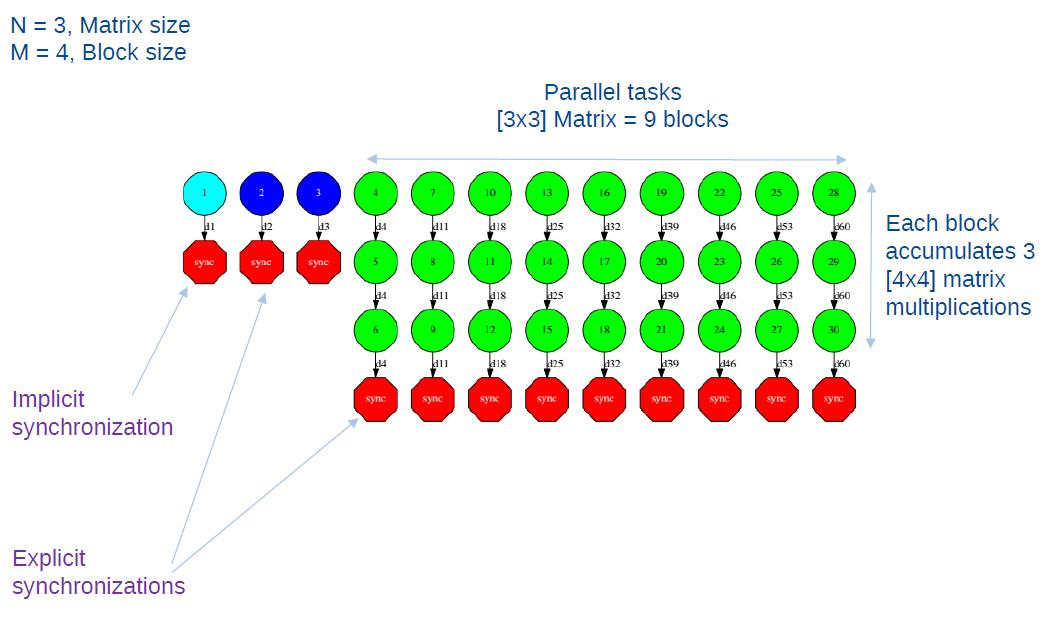
\includegraphics[width=1.0\textwidth]{./Sections/6_Bindings/Figures/matmul.jpeg}
    %\caption{Matmul Execution Graph.}
    %\label{fig:BLAST_workflow}
\end{figure}

\subsection{Python}

COMPSs features a binding for Python 2.x applications. The next subsections explain how to program a Python 
application for COMPSs and how to configure the binding library.

\subsubsection{Programming Model}

\paragraph{Task Selection}

Like in the case of the Java language, a COMPSs Python application is a sequential program that contains calls 
to tasks. In particular, the user can select as a task:

\begin{itemize}
 \item Functions
 \item Instance methods: methods invoked on objects.
 \item Class methods: static methods belonging to a class.
\end{itemize}

Regarding task selection, in Python it is not done by means of an annotated interface but with the use of 
Python decorators. In particular, the user needs to add, before the definition of the function/method, 
a @task decorator that describes the task.

As an example, let us assume that the application calls a function func, which receives a string parameter 
containing a file name and an integer parameter. The code of func updates the file.

\begin{lstlisting}[language=python]
my_file = 'sample_file.txt'
func(my_file, 1)
\end{lstlisting}

In order to select {\it func} as a task, the corresponding {\it @task} decorator needs to be placed right 
before the definition of the function, providing some metadata about the parameters of that function. 
The metadata corresponding to a parameter is specified as an argument of the decorator, whose name is 
the formal parameter’s name and whose value defines the type and direction of the parameter. 
The parameter types and directions can be:

\begin{itemize}
 \item Types: {\it primitive types} (integer, long, float, boolean), {\it strings}, {\it objects} (instances of user-defined classes, dictionaries, lists, tuples, complex numbers) and {\it files} are supported.
 \item Direction: it can be read-only ({\it IN} - default), read-write ({\it INOUT}) or write-only ({\it OUT}).
\end{itemize}

COMPSs is able to automatically infer the parameter type for primitive types, strings and objects, 
while the user needs to specify it for files. On the other hand, the direction is only mandatory for 
{\it INOUT} and {\it OUT} parameters. Thus, when defining the parameter metadata in the {\it @task} 
decorator, the user has the following options:

\begin{itemize}
 \item {\it INOUT}: the parameter is read-write. The type will be inferred.
 \item {\it OUT}: the parameter is write-only. The type will be inferred.
 \item {\it FILE}: the parameter is a file. The direction is assumed to be {\it IN}.
 \item {\it FILE\_INOUT}: the parameter is a read-write file.
 \item {\it FILE\_OUT}: the parameter is a write-only file.
\end{itemize}
     
Consequently, please note that in the following cases there is no need to include an argument in 
the {\it @task} decorator for a given task parameter:

\begin{itemize}
 \item Parameters of primitive types (integer, long, float, boolean) and strings: the type of these 
       parameters can be automatically inferred by COMPSs, and their direction is always {\it IN}.
 \item Read-only object parameters: the type of the parameter is automatically inferred, and the 
       direction defaults to {\it IN}.
\end{itemize}
 
Continuing with the example, in the following code snippet the decorator specifies that {\it func} 
has a parameter called {\it fi}, of type {\it FILE} and {\it INOUT} direction. Note how the second 
parameter, {\it i}, does not need to be specified, since its type (integer) and direction ({\it IN}) 
are automatically inferred by COMPSs.

\begin{lstlisting}[language=python]
from pycompss.api.task import task
from pycompss.api.parameter import *
%*{\bf @task }*)(f = FILE_INOUT)
def func(f, i):
     fd = open(f, ‘r+’)
     ...
\end{lstlisting}

If the function or method returns a value, the programmer must specify the type of that value using 
the {\it returns} argument of the {\it @task} decorator:

\begin{lstlisting}[language=python]
@task(%*{\bf returns }*) = int)
def ret_func():
     return 1
\end{lstlisting}

For tasks corresponding to instance methods, by default the task is assumed to modify the callee object 
(the object on which the method is invoked). The programmer can tell otherwise by setting the 
{\it isModifier} argument of the {\it @task} decorator to {\it False}.

\begin{lstlisting}[language=python]
class MyClass(object):
    ...
    @task(%*{\bf isModifier }*) = False)
    def instance_method(self):
        ... # self is NOT modified here
\end{lstlisting}

The programmer can also mark a task as a high-priority task with the {\it priority} argument of the 
{\it @task} decorator. This way, when the task is free of dependencies, it will be scheduled before 
any of the available low-priority (regular) tasks. This functionality is useful for tasks that are in 
the critical path of the application’s task dependency graph.

\begin{lstlisting}[language=python]
@task(%*{\bf priority }*) = True)
def func():
    ...
\end{lstlisting}

Table \ref{tab:task_decorator_arguments} summarizes the arguments that can be found in the @task decorator.

\begin{longtable}{| p{0.31\textwidth} | p{0.69\textwidth} |}
\hline
\multicolumn{1}{|c|}{{\bf Argument }}    &  \multicolumn{1}{c|}{{\bf Value }}\\
\hline
\multirow{5}{*}{Formal parameter name}  &  - INOUT: read-write parameter, all types except file (primitives, strings, objects). \\
& - OUT: read-write parameter, all types except file (primitives, strings, objects). \\
& - FILE: read-only file parameter. \\
& - FILE\_INOUT: read-write file parameter. \\
& - FILE\_OUT: write-only file parameter. \\
\hline
returns & int (for integer and boolean), long, float, str, dict, list, tuple, user-defined classes \\
\hline
isModifier &  True (default) or False \\
\hline
priority  & True or False (default) \\
\hline
\caption{Arguments of the {\it @task} decorator.}
\label{tab:task_decorator_arguments}
\end{longtable}


\paragraph{Main Program}
The main program of the application is a sequential code that contains calls to the selected tasks. 
In addition, when synchronizing for task data from the main program, 
there exist two API functions that need to be invoked:

\begin{itemize}
 \item {\it compss\_open(file\_name, mode = 'r')}: similar to the Python {\it open()} call. It synchronizes
       for the last version of file {\it file\_name} and returns the file descriptor for that synchronized
       file. It can receive an optional parameter {\it mode}, which defaults to '{\it r}', containing the
       mode in which the file will be opened (the open modes are analogous to those of
       Python {\it open()}).
 \item {\it compss\_wait\_on(obj, to\_write = True)}: synchronizes for the last version of object {\it obj}
       and returns the synchronized object. It can receive an optional boolean parameter
       {\it to\_write}, which defaults to {\it True}, that indicates whether the main program will modify the
       returned object.
\end{itemize}

To illustrate the use of the aforementioned API functions, the following example first invokes a task 
{\it func} that writes a file, which is later synchronized by calling {\it compss\_open()}. 
Later in the program, an object of class {\it MyClass} is created and a task method {\it method} 
that modifies the object is invoked on it; the object is then synchronized with {\it compss\_wait\_on()}, 
so that it can be used in the main program from that point on.

\begin{lstlisting}[language=python]
from pycompss.api.api import compss_open, compss_wait_on

my_file = 'file.txt'
func(my_file)
fd = %*{\bf compss\_open}*)(my_file)
...

my_obj = MyClass()
my_obj.method()
my_obj = %*{\bf compss\_wait\_on}*)(my_obj)
...
\end{lstlisting}

The corresponding task selection for the example above would be:

\begin{lstlisting}[language=python]
@task(f = FILE_OUT)
def func(f):
    ...
    
    class MyClass(object):
        ...
        
        @task()
        def method(self):
            ... # self is modified here
\end{lstlisting}

Table \ref{tab:python_api_functions} summarizes the API functions to be used in the main program of a COMPSs Python application.

\begin{longtable}{| p{0.30\textwidth} | p{0.7\textwidth} |}
\hline
\multicolumn{1}{|c|}{{\bf Function }}    &  \multicolumn{1}{c|}{{\bf Use }}\\
\hline
compss\_open(file\_name, mode = 'r') & Synchronizes for the last version of a file and returns its file descriptor. \\
\hline
compss\_wait\_on(obj, to\_write = True) & Synchronizes for the last version of an object and returns it. \\
\hline
\caption{COMPSs Python API functions.}
\label{tab:python_api_functions}
\end{longtable}


\subparagraph{Future Objects}
If the programmer selects as a task a function or method that returns a value, that value is not 
generated until the task executes. However, in order to keep the asynchrony of the task invocation, 
COMPSs manages future objects: a representant object is immediately returned to the main program when 
a task is invoked.

\begin{lstlisting}[language=python]
@task(%*{\bf returns }*) = MyClass)
def ret_func():
    return MyClass(...)

...

# %*{\bf o }*) is a future object
o = ret_func()
\end{lstlisting}

The future object returned can be involved in a subsequent task call, and the COMPSs runtime will automatically 
find the corresponding data dependency. In the following example, the future object o is passed as a parameter 
and callee of two subsequent (asynchronous) tasks, respectively:

\begin{lstlisting}[language=python]
# %*{\bf o }*) is a future object
o = ret_func()

...

another_task(o)

...

o.yet_another_task()
\end{lstlisting}

In order to synchronize the future object from the main program, the programmer proceeds in the same way 
as with any object updated by a task:

\begin{lstlisting}[language=python]
# %*{\bf o }*) is a future object
o = ret_func()

...

o = compss_wait_on(o)
\end{lstlisting}
                         
The future object mechanism is applied to primitive types, strings and objects (including the Python 
built-in types list, dictionary and tuple).

It is important to note that, for instances of user-defined classes, the classes of these objects 
should have an empty constructor, otherwise the programmer will not be able to invoke task instance 
methods on those objects:
                                   
\begin{lstlisting}[language=python]
class MyClass(object):
    def __init__(self): # empty constructor
        ...
        
    ...

o = ret_func()

# invoking a task instance method on a future object can only
# be done when an empty constructor is defined in the object's
# class
o.yet_another_task()
\end{lstlisting}

\paragraph{Important Notes}
For the COMPSs Python binding to function correctly, the programmer should not use relative imports 
in her code. Relative imports can lead to ambiguous code and they are discouraged in Python, as explained in:

\begin{lstlisting}[language=html]
http://docs.python.org/2/faq/programming.html#what-are-the-best-practices-for-using-import-in-a-module
\end{lstlisting}

\subsubsection{Application Execution}
The next subsections describe how to execute applications with the COMPSs Python binding.

\paragraph{Environment}
The following environment variables must be defined before executing a COMPSs Python application:

JAVA\_HOME: Java JDK installation directory (e.g. /usr/lib/jvm/java-6-openjdk/)

\paragraph{Command}

In order to run a Python application with COMPSs, the script runcompssext can be used, like for 
Java and C/C++ applications. An example of an invocation of the script is:

\begin{lstlisting}[language=bash]
> runcompssext
  --lang=python
  --app=$TEST_DIR/test.py
  --classpath=$TEST_DIR
  --library_path=/home/user/libdir
  --cline_args="arg1 arg2"
  --project=$TEST_DIR/project.xml
  --resources=$TEST_DIR/resources.xml
  --tracing=true
\end{lstlisting}

The options of the script are:

\begin{lstlisting}[language=bash]
  --lang=python
  --app=<path>: path to the .py file containing the main program.
  --classpath=<path>: path/s where to search for the application’s Python modules. The default value is the current directory.
  --library_path=<path>: path/s where to search for libraries that are not in a standard path. The default value is the variable $LD_LIBRARY_PATH.
  --cline_args=<args>: arguments to pass to the application.
  --project=<proj_file>: path of the project XML file.
  --resources=<res_file>: path of the resources XML file.
  --tracing=<true | false>: generate execution traces. Default is false.
\end{lstlisting}